\scanpage{41}
\unsure{\S}\quad\deleted{\uline{Systèmes linéaires et} \unsure{schémas}} \uline{Schémas de Brauer}

\uline{Séveri}

\uline{Déf} \uline{Schéma de Brauer Séveri} \deleted{\unsure{X}} $P/S$ : il devient un fibré projectif loc. fppf

\deleted{\uline{Remarques}}

\uline{Proposition} 1 Un tel $P$ est \uline{projectif} et lisse sur $S$. Le faisceau \deleted{\unsure{\Omega}} $\underline\omega_{X/S}^{-1}$ est ample rel. à $S$.

\uline{Proposition} 2 \deleted{Si $P/S$ a une section, alors $P$} \inserted{Pour que $P$ soit un fibré projectif,} il \uline{\unsure{ft} et suff.} qu'il existe sur $P$ un faisceau inversible \deleted{\unsure{dont les}} de degré 1 sur chaque fibre, ou ce qui revient au $=$, tel que
\[
\underline L^{\otimes(r+1)}\otimes\underline\Omega^r_{X/S}
\]
soit isomorphe à l'image inverse d'un faisceau inv. sur $S$.
\margin{\figure{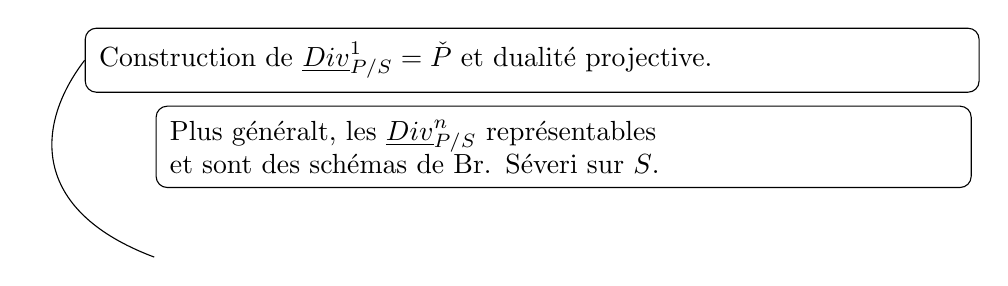
\begin{tikzpicture}[x=1cm,y=1cm]
\node[draw,rounded corners,align=left,text width=11cm,inner sep=5pt] (a) at (0,1.1) {\uline{Construction de} $\underline{\operatorname{Div}}^1_{P/S}=\check P$ et \uline{dualité projective}.};
\node[draw,rounded corners,align=left,text width=10cm,inner sep=5pt] (b) at (.4,0) {Plus généralt, les $\underline{\operatorname{Div}}^{\unsure{n}}_{P/S}$ représentables\par et sont des schémas de Br. Séveri sur $S$.};
\draw (a.west)..controls(-6.3,.3)and(-6.4,-.8)..(-4.8,-1.4);
\end{tikzpicture}}}
\margin{\figure{\begin{tikzpicture}\draw (0,0)--(-.15,0)--(-.15,-2.7)--(0,-2.7);\end{tikzpicture}}}

\unsure{Ca} signifie \unsure{encore} que le résultat de classification donné au $\mathrm N^\circ1$ pour $\operatorname{Pic}(P)$ est valable $\ldots$

\margin{\uline{Corollaire} Cas d'un schéma de base régulier.}

\uline{Proposition} 3 Si $P$ admet une section \inserted{sur $S$}, c'est un fibré projectif : utiliser la théorie de descente \inserted{et dualité des projectifs}.
\margin{\figure{\begin{tikzpicture}\draw (.15,0)--(0,0)--(0,-.8)--(.15,-.8);\end{tikzpicture}}}
\unsure{Évident que aussi} si $\forall$ Module loc. libre sur $S$ est libre (p.ex. $S$ local) \deleted{\unsure{schéma régulier de dim 1} \unsure{spectre} d'un anneau \inserted{principal}}
\mspage{40}
